\documentclass[10pt]{article}
\usepackage[a4paper,margin=1.8cm]{geometry}
\usepackage[T1]{fontenc}
\usepackage{lmodern}
\usepackage{microtype}
\usepackage{booktabs}
\usepackage{longtable}
\usepackage{tabularx}
\usepackage{graphicx}
\usepackage{pdflscape}
\usepackage[numbers,sort&compress]{natbib}
\usepackage[colorlinks=true,allcolors=blue]{hyperref}
\usepackage{caption}
\usepackage{lineno}
\graphicspath{{figures/}}
\newcommand{\BenchmarkN}{85}
\newcommand{\ClassicalMAE}{0.785}
\newcommand{\PIMDMAE}{0.205}
\newcommand{\PreviousMAE}{0.239}
\newcommand{\NarrowMAE}{0.214}
\newcommand{\SMDMAE}{0.202}
\newcommand{\SolvAIMAE}{0.197}
\newcommand{\NestedMAE}{0.199}
\newcommand{\RepeatMean}{0.204}
\newcommand{\RepeatSD}{0.005}
\newcommand{\NestedRepeatMean}{0.209}
\newcommand{\NestedRepeatSD}{0.003}
\newcommand{\FamilyMAE}{0.240}
\newcommand{\ScaffoldMAE}{0.241}
\newcommand{\MolSolvN}{350,391}
\newcommand{\ConfSolvN}{39,878}

\newcolumntype{Y}{>{\raggedright\arraybackslash}X}

\title{Supplementary Information\\[4pt]\large Distilling solvation physics into AI for simulation-free hydration free energies}
\author{Gal Oren and Michael Levitt}
\date{}

\begin{document}
\linenumbers
\maketitle

\section*{Supplementary overview}

This document reports the complete validation record supporting SolvAI. It separates the deployable structure-only model from candidate calculations that require simulation at inference, and it preserves non-improving physical-supervision experiments without making them the main narrative. All numerical values originate from \path{results/paper_metrics.json}; the corresponding molecule-level predictions are distributed with the repository.

\section*{Supplementary Table 1: complete primary comparison}

\begin{table}[h]
\centering
\small
\begin{tabular}{lcccc}
\toprule
Method & Simulation at inference & Random OOF & Family holdout & Scaffold holdout \\
\midrule
Classical ARROW & yes & 0.785 & -- & -- \\
ARROW/PIMD8 & yes & 0.205 & -- & -- \\
Previous structure-only & no & 0.239 & -- & -- \\
Narrow response & no & 0.214 & -- & -- \\
+ SMD(water) & no & 0.202 & -- & -- \\
SolvAI: + ConfSolv response & no & 0.197 & 0.240 & 0.241 \\
Nested feature selection & no & 0.199 & -- & -- \\
\bottomrule
\end{tabular}

\caption{MAE in kcal mol$^{-1}$. A dash denotes a comparison that was not defined for that fixed artifact. Only rows marked ``no'' satisfy the deployment requirement.}
\end{table}

\section*{Supplementary Table 2: independent split repeats}

\begin{center}
\begin{tabular}{lrrrrrrr}
\toprule
Procedure & Split 1 & Split 2 & Split 3 & Split 4 & Split 5 & Mean & SD \\
\midrule
Fixed SolvAI & 0.2074 & 0.1979 & 0.2085 & 0.2060 & 0.1991 & 0.2038 & 0.0049 \\
Nested selection & 0.2057 & 0.2067 & 0.2113 & 0.2076 & 0.2117 & 0.2086 & 0.0027 \\
\bottomrule
\end{tabular}
\end{center}

The five split seeds were 314159, 271828, 161803, 141421 and 173205. Each row is a complete five-fold OOF evaluation. No split was removed or replaced on the basis of its result.

\section*{Supplementary Table 3: master experiment table}

\begin{landscape}
\footnotesize
\setlength{\tabcolsep}{3pt}
\begin{longtable}{p{2.8cm}p{4.0cm}p{3.1cm}p{2.4cm}p{1.8cm}p{1.5cm}p{4.3cm}p{1.6cm}}
\toprule
Experiment & Scientific hypothesis & Data or response source & Inference & Leakage & OOF MAE & Interpretation & Retained \\
\midrule
\endfirsthead
\toprule
Experiment & Scientific hypothesis & Data or response source & Inference & Leakage & OOF MAE & Interpretation & Retained \\
\midrule
\endhead
Previous structure-only & Molecular fingerprints and descriptors directly encode hydration & public hydration + RDKit/Morgan & SMILES & strict & 0.23861 & Establishes the pre-distillation baseline & yes, as base \\
Narrow response & Compact physical axes regularize the endpoint & CombiSolv-QM, Abraham, OpenFF, GBn2 & SMILES & strict & 0.21362 & Broad but targeted response supervision transfers & yes \\
SMD water response & A water-specific continuum target supplies missing solvent response & MolSolv SMD(water) & SMILES & strict & 0.20161 & Largest single aligned gain & yes \\
ConfSolv response & Conformer reweighting and response distributions add complementary information & ConfSolv H$_2$O & SMILES & strict & 0.19705 & Closes the remaining point-estimate gap to PIMD8 & yes \\
Nested block selection & Improvement survives selection confined to training folds & same three feature blocks & SMILES & nested strict & 0.19931 & Confirms the crossing without outer-test block choice & confir\-matory \\
PIMD8 residual correction & Remaining PIMD8 error is learnable & ARROW/PIMD8 + experiment & test-molecule PIMD8 & nested & 0.18682 & Ceiling result; non-deployable & no \\
OpenFE diagnostics & Simulation convergence and component structure add information & explicit-water ASFE archive & SMILES after distillation & strict & 0.20575 & Non-improving matched screen & no \\
MLFF hierarchy & Multiple force-field estimates span missing physics & published MLFF hydration values & SMILES after distillation & strict & 0.20109 & Non-improving matched screen & no \\
DES370K/SAPT & Pair interaction components improve water response & water-dimer SAPT subset & SMILES after distillation & strict & 0.20993 & Pair physics was insufficiently aligned to the endpoint & no \\
GNNIS force response & Learned explicit-water forces give a useful latent response & public force-matched model & structure & strict & 0.20794 & Static distilled response did not improve & no \\
Lambda-aware implicit response & Coupling-dependent potential transfers to hydration & public potential & structure & strict & 0.20974 & Non-improving & no \\
Phase-space response & Structural dynamics supply complementary response information & explicit-solvent phase-space averages & SMILES after distillation & strict & 0.21894 & Non-improving & no \\
G-NequIP hierarchy & 3D solvation representations improve transfer & gas/SMD 3D model & conformer only & strict & 0.22276 & Non-improving & no \\
ConfSolv graph latent & Learned latent is richer than summary targets & ConfSolv graph encoder & SMILES & strict & 0.21219 & Compact response moments transferred better & no \\
ConfSolv FFN latent & Feed-forward hidden state improves endpoint & ConfSolv encoder & SMILES & strict & 0.21548 & Non-improving & no \\
Multi-$\lambda$ response & A predicted alchemical curve is a better intermediate than one scalar & three-point PIMD2 response & SMILES after distillation & outer-fold strict & 0.20136 & Response errors remain too large & no \\
Fidelity hierarchy & Classical, NQE and PIMD heads order the physical target & ARROW classical/PIMD labels & SMILES after distillation & outer-fold strict & 0.21474 & Sparse aligned labels do not yet transfer precisely & no \\
Integrated response curve & Predicted $\mathrm{d}H/\mathrm{d}\lambda$ can be integrated directly & three-point PIMD2 response & SMILES after distillation & outer-fold strict & 1.51356 & Identifies structure-to-response accuracy as bottleneck & no \\
Selective simulation & Routing difficult molecules preserves accuracy at lower cost & PIMD8 fallback & PIMD8 for selected inputs & explor\-atory & varies & Outside final deployment objective; archived for completeness & no \\
\bottomrule
\end{longtable}
\end{landscape}

\section*{Extended Data Figures}

\begin{figure}[p]
\centering
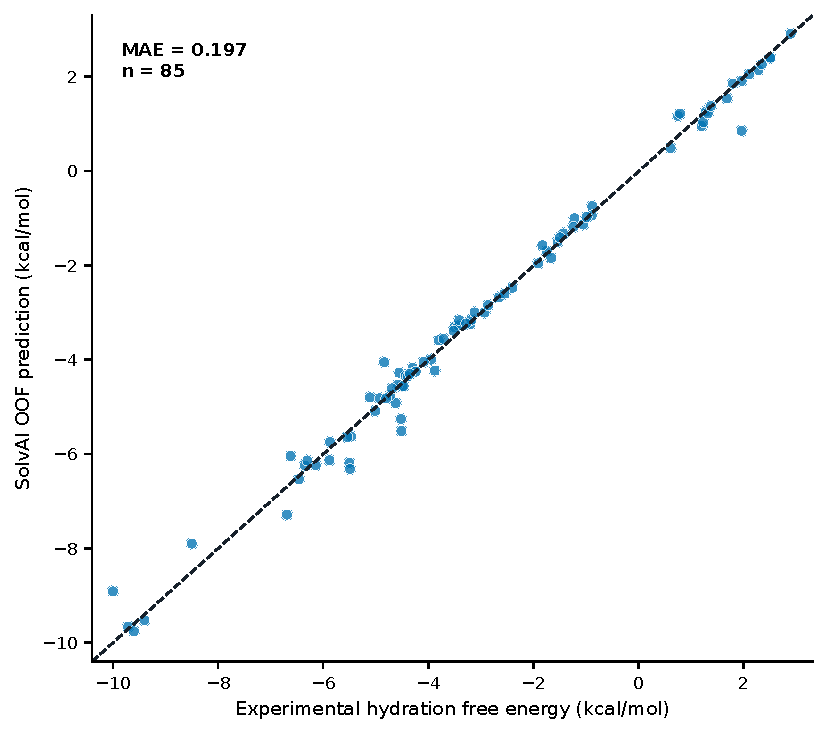
\includegraphics[width=0.78\textwidth]{extended_data_1_parity.pdf}
\caption{\textbf{Extended Data Figure 1 | Experimental and strict OOF predictions.} Each point is produced by a model that did not receive that molecule's experimental target. The diagonal denotes equality.}
\end{figure}

\begin{figure}[p]
\centering
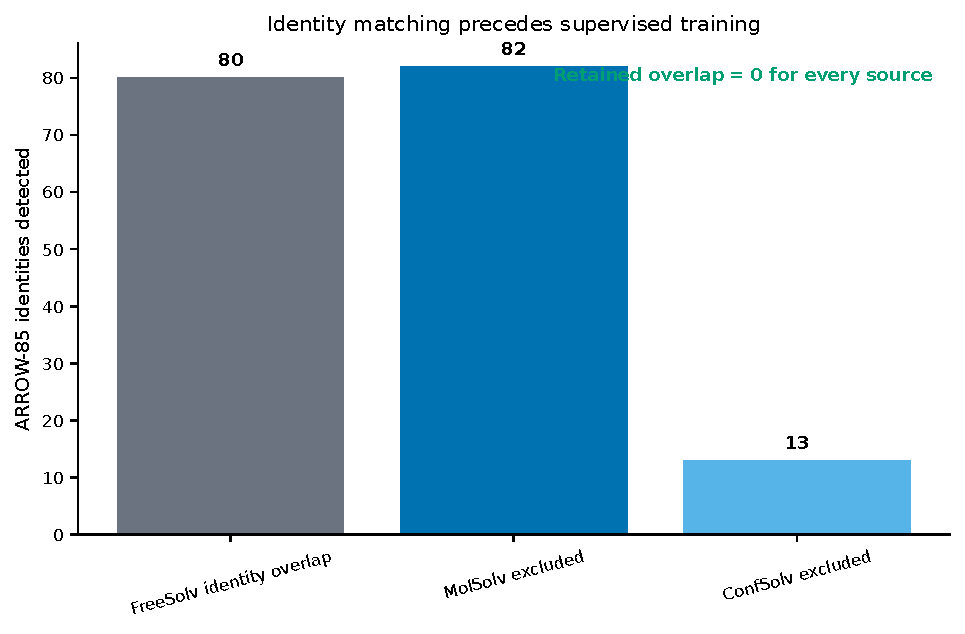
\includegraphics[width=0.85\textwidth]{extended_data_2_identity_audit.pdf}
\caption{\textbf{Extended Data Figure 2 | Benchmark identity analysis and exclusions.} Eighty benchmark connectivities are also present in FreeSolv. Independent global exclusion removed 82 exact MolSolv structures and 13 ConfSolv connectivities; no retained training source overlaps ARROW-85. Counts are identity detections and need not share a provenance.}
\end{figure}

\begin{figure}[p]
\centering
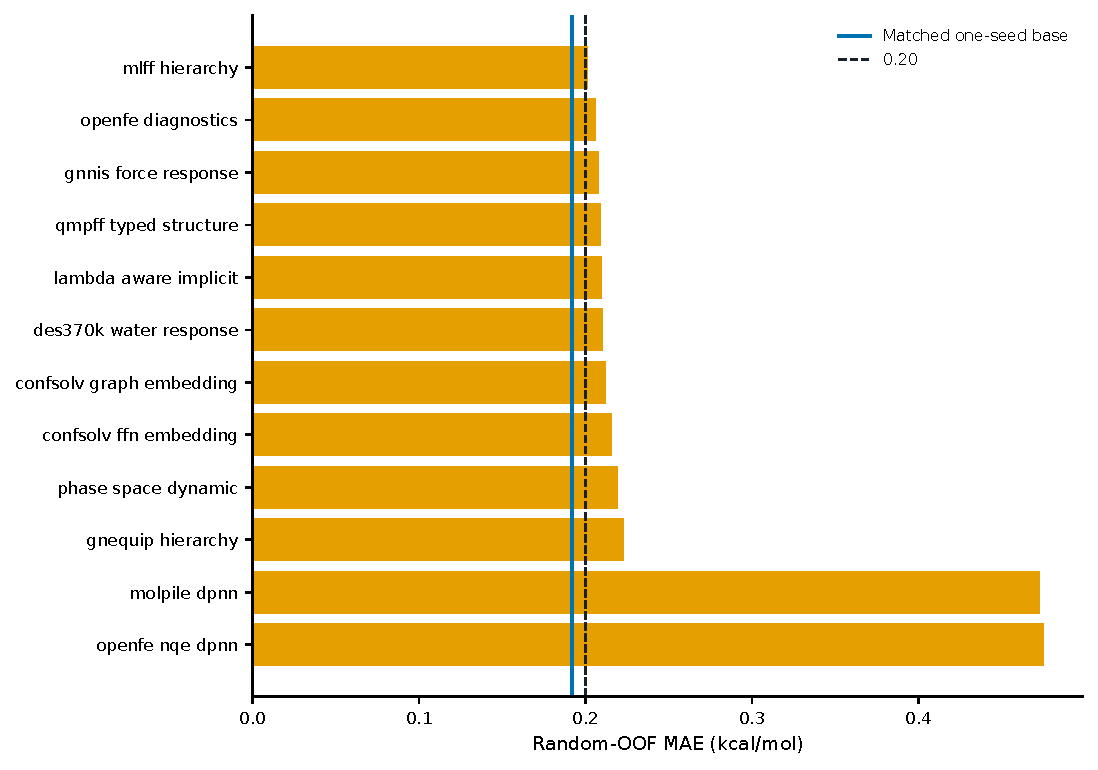
\includegraphics[width=0.88\textwidth]{extended_data_3_alternative_supervision.pdf}
\caption{\textbf{Extended Data Figure 3 | Alternative physical supervision routes.} Random-OOF MAEs from matched or otherwise frozen screens. These experiments test transfer utility, not the intrinsic quality of each physical method. The matched one-seed base is shown in blue.}
\end{figure}

\begin{figure}[p]
\centering
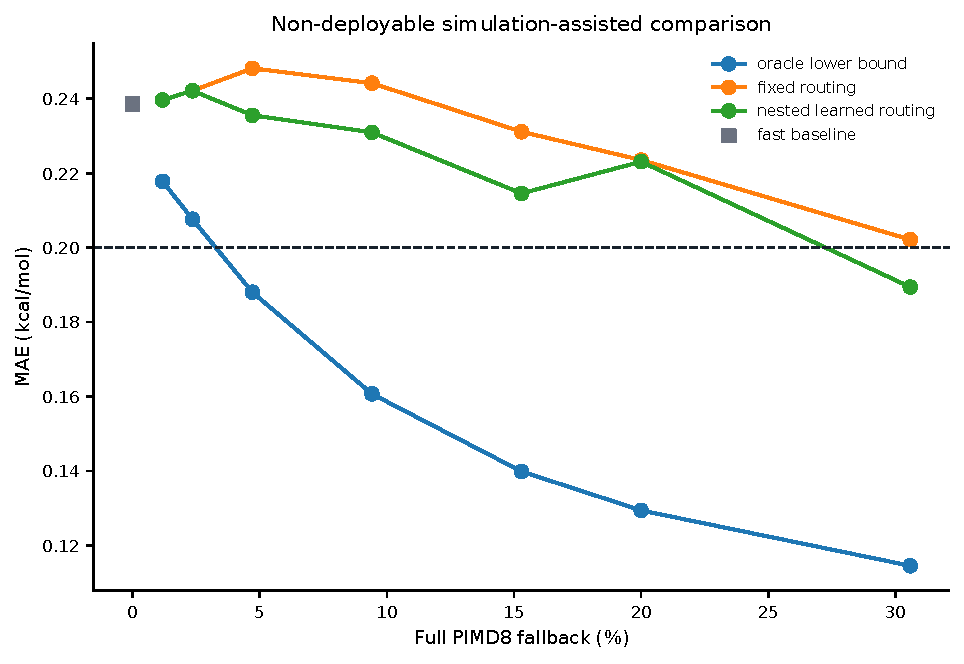
\includegraphics[width=0.82\textwidth]{extended_data_4_simulation_assisted.pdf}
\caption{\textbf{Extended Data Figure 4 | Non-deployable simulation-assisted comparisons.} Archived selective-PIMD analyses show an oracle lower bound and learned routing under the original random OOF regime. They require PIMD for test molecules and are excluded from SolvAI and all headline claims.}
\end{figure}

\begin{figure}[p]
\centering
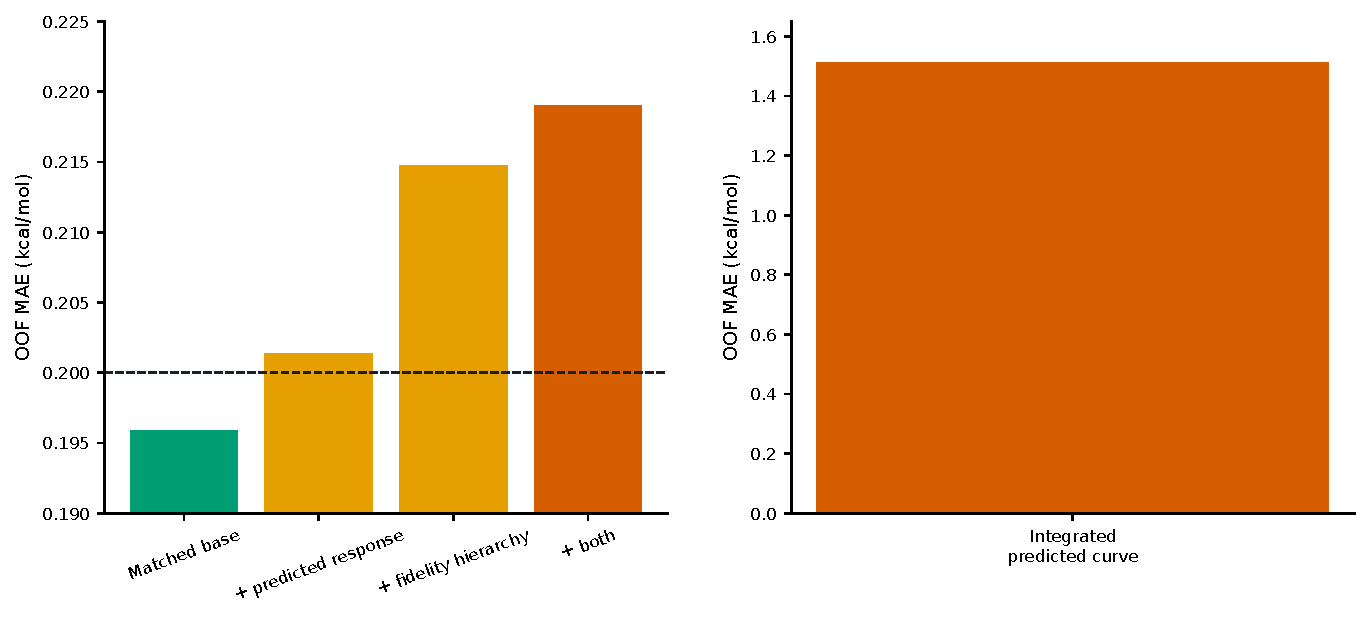
\includegraphics[width=0.94\textwidth]{extended_data_5_multilambda.pdf}
\caption{\textbf{Extended Data Figure 5 | Multi-$\lambda$ response distillation.} Predicted PIMD2 response, fidelity hierarchy and their combination all worsened the matched structure-only endpoint. Direct integration of the predicted response was substantially less accurate.}
\end{figure}

\begin{figure}[p]
\centering
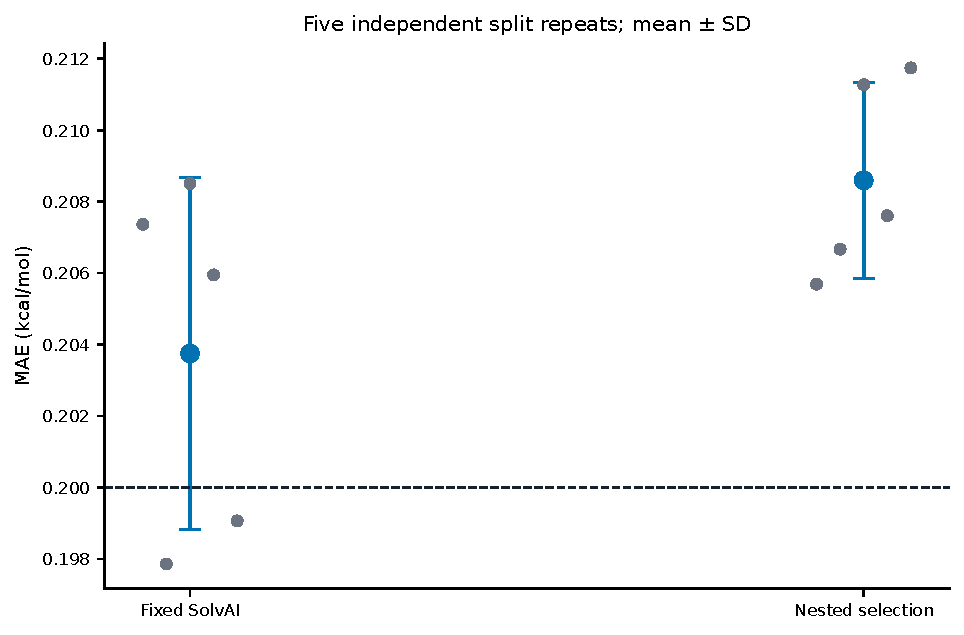
\includegraphics[width=0.82\textwidth]{extended_data_6_repeat_statistics.pdf}
\caption{\textbf{Extended Data Figure 6 | Independent partition sensitivity.} Points show the five complete repeat MAEs; markers and whiskers show mean and one sample standard deviation.}
\end{figure}

\begin{figure}[p]
\centering
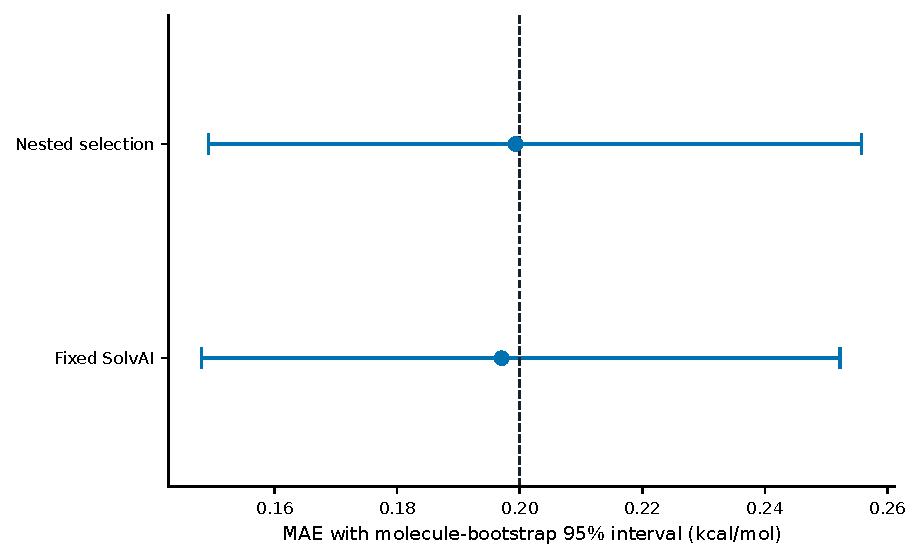
\includegraphics[width=0.82\textwidth]{extended_data_7_bootstrap.pdf}
\caption{\textbf{Extended Data Figure 7 | Molecule-bootstrap uncertainty.} Point estimate and 95\% percentile interval from 100,000 resamples. The width reflects the small, heterogeneous reference set.}
\end{figure}

\begin{figure}[p]
\centering
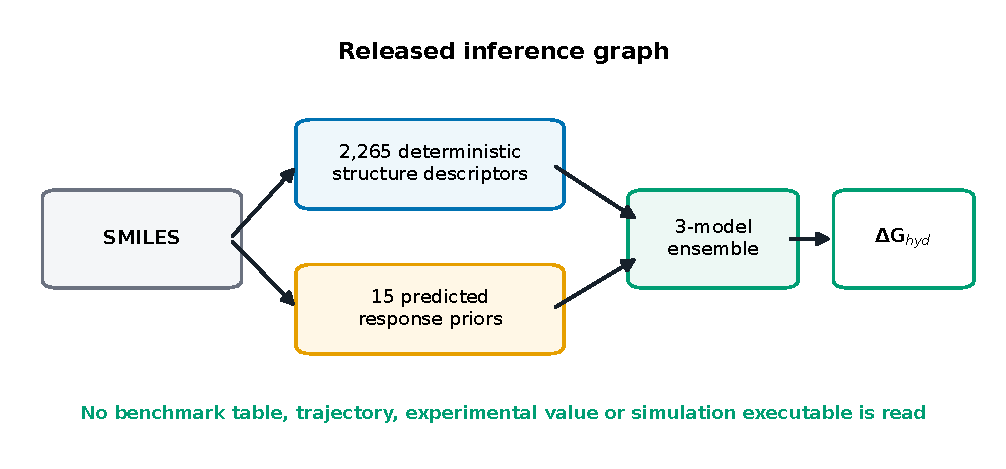
\includegraphics[width=0.98\textwidth]{extended_data_8_artifact_audit.pdf}
\caption{\textbf{Extended Data Figure 8 | Released inference graph.} The public artifact receives SMILES, computes deterministic descriptors and structure-derived response priors, and returns an ensemble prediction. Runtime source inspection and schema validation confirm that no benchmark table, trajectory or experimental label is read.}
\end{figure}

\clearpage
\section*{Supplementary Methods}

\subsection*{Teacher-source filtering}

For MolSolv, all reference-set connectivity matches were removed before a deterministic size-stratified sample was selected: all eligible molecules with at most ten heavy atoms and one eighth, chosen by SHA-256, with 11--18 heavy atoms. This yielded 350,391 rows and 348,587 unique connectivities. For ConfSolv, H$_2$O records were grouped by resolved neutral connectivity after removing all benchmark matches. Ensemble and lowest-energy-conformer solution values were converted from kJ mol$^{-1}$ to kcal mol$^{-1}$; response summaries were calculated within connectivity. No benchmark target entered either operation.

The public endpoint set combined benchmark-disjoint hydration values and retained 1,280 labels using the frozen source-quality mask: membership in the earlier curated table or at least two source measurements. Experimental endpoint rows had unit weight; reference-set outer-training rows had weight three. This weighting and every tree hyperparameter were fixed before confirmatory repeated splits.

\subsection*{Family and scaffold folds}

Chemical families were assigned by deterministic structural rules used throughout the campaign. Grouped validation ensures that all members of an assigned family occupy the same held-out partition. Scaffold groups were constructed from the frozen scaffold field; acyclic and small-ring structures were balanced across five groups while preserving identical scaffold membership. These tests are deliberately harder than random OOF and are reported even though neither reaches 0.20 kcal mol$^{-1}$.

\subsection*{Artifact verification}

The model manifest stores SHA-256, byte length and role for each of seven executable artifacts and the model card. Verification checks every hash, then runs ethanol and benzene from SMILES through the public API. Expected predictions are $-5.020248$ and $-0.893576$ kcal mol$^{-1}$, respectively, with absolute tolerance $2\times10^{-6}$. The test starts no simulator and requires no benchmark file.

\subsection*{Runtime protocol}

Cold latency was measured in a fresh Python process. Warm single-molecule latency was measured five times after one warm-up call in the same process. Batch throughput used three runs of 32 SMILES. Timing spans canonicalization, descriptor construction, both D-MPNN processes, all tree teachers and the endpoint ensemble. Median warm latency was 17.522 s and p95 was 17.627 s; median batch time was 17.911 s (0.560 s per molecule). Peak resident memory was 155,408 KiB. The benchmark JSON records exact package, CPU and accelerator information.

\end{document}
